\title{Emojis and Weather}
\author{
        Darryl Hannan \\
                Villanova University
\and
	Emma Chin \\
		Villanova University
\and
	Matt Mador \\
		Villanova University
}
\date{\today}

\documentclass[12pt]{article}
\usepackage{graphicx}
\usepackage{float}
\graphicspath{{images/}}

\begin{document}
\maketitle

\begin{abstract}
A significant amount of research has been done analyzing the impact weather has on emotional states. Most of these studies are survey based, and therefore have a small sample size. Here, we seek to overcome this problem through the use of social media. We analyze tweets from various geographic locations, extracting emojis. We use the distribution of emojis to represent the emotional state of a population. We use these representations to train a machine learning classifier that predicts the weather. Our model is approximately 88\% accurate, providing support for the link between weather and mood.
\end{abstract}

\section{Introduction}
The impact that weather has on mood is well established. Spasova (2011) found that abrupt transitions to unfavorable weather conditions has a negative effect on emotion.\cite{Spasova2011} Keller et al. (2005) found that time spent in pleasant weather results in better mood and improved memory.\cite{Keller2005} Some effects are more serious; seasonal effective disorder occurs occurs during winter months, when the days are shortest, and can result in serious cases depression.\cite{Melrose2015}

The effect that weather has on emotions varies significantly among individuals.\cite{Spasova2011} Therefore, large sample sizes are needed to discover correlations between specific weather patterns and emotional states. Traditionally, the only way to study this set of phenomena was through survey based methods, resulting in small sample sizes. We attempt to overcome this problem through the use of Twitter. By analyzing the emotions expressed in tweets for a given geographic location, we obtain an approximation of the collective emotional state of the population. This method also makes it significantly less expensive to collect data. By running the collection program on a server, we can continuously collect data indefinitely.

\section{Related Work}
Park et al. (2013) also utilize Twitter to gather emotional data.\cite{Park2013} They use a linear regression model to predict various variables such as temperature, humidity, and precipitation. Our approach differs in that Park et al. perform sentiment analysis on the tweets, whereas we use emojis to represent sentiment. By using emojis, we require significantly less preprocessing and impose less structure on the emotional representation that the model ultimately learns.

Baylis et al. (2017) use both Twitter and Facebook to collect emotional data. Using more than 3.5 billion social media posts in their model.\cite{Baylis2017} Their weather variable, referred to as cloud cover, is similar to the variable that we predict in our model. The primary difference in our model again lies in the use of emojis.

\section{Data}

\subsection{Emotion Data}
We collect tweets from 21 cities using Twitter's Streaming API via Tweepy\footnote{http://www.tweepy.org/}, targeting locations with high populations in order to maximize the number of data points. We preselected a list of 75 emojis that commonly represent various emotional states (Figure \ref{fig:emojis}). As each tweet is received, we count the occurrences of each emoji in the tweet. We collect data in 2 hour intervals. The distribution of emojis for each interval is represented in a vector format, where each dimension of the vector contains the count of a given emoji. Data was collected over a period of approximately 2 weeks.

\begin{figure}[t]
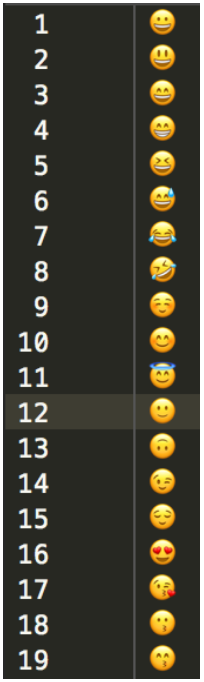
\includegraphics[scale=0.7]{emojiexample}
\centering
\caption{Example of emojis that we extract from tweets}
\label{fig:emojis}
\end{figure}

\subsection{Weather Data}
We access weather data for each location through the OpenWeatherMap API. We use PyOWM\footnote{https://github.com/csparpa/pyowm}, an open-source python wrapper, to simplify API calls. Weather data is collected concurrently with Twitter data. At the end of each 2 hour interval, we collect the current atmospheric condition in each city. Examples of atmospheric conditions include rain, snow, clear, etc. In the data we collected, there are 8 classes of conditions: clouds, clear, rain, drizzle, mist, fog, snow, haze, and dust.

\subsection{Preprocessing}\label{preprocessing}
One issue that we encountered was that some of the emoji vectors were extremely sparse. In some cities, such as Nashville, almost every vector only had a few emojis. Therefore, we only include vectors in which the sum of its elements is greater than 40. For classification, each atmospheric condition is represented using a number from the range 0-7. In the case of binary classification, we consider clear to be a positive weather condition and represent it with a 0. We consider all other conditions to be negative and represent these using a 1. Our final data set consisted of 977 data pairs.

\section{Methods}
We compare five learning algorithms on our classification tasks: ZeroR, a Gaussian Mixture Model (GMM), an Artificial Neural Network (ANN), a Decision Tree, and Naive Bayes. We use ZeroR to establish a baseline, and we use a GMM to evaluate how our data clusters. We implement all models, with the exception of the ANN, using Scikit-Learn\footnote{http://scikit-learn.org/stable/}. The models do not benefit significantly from modifying parameters. Results can be achieved by leaving them at their default values.

Our ANN is implemented using Keras\footnote{https://keras.io/}. The model architecture can be seen in Figure \ref{fig:neuralnet}. We use a ReLU activation function, binary crossentropy to evaluate our loss, and adam as our optimizer\cite{Nair2010}\cite{Kingma2015}. The model is trained for 20 epochs.

\begin{figure}[H]
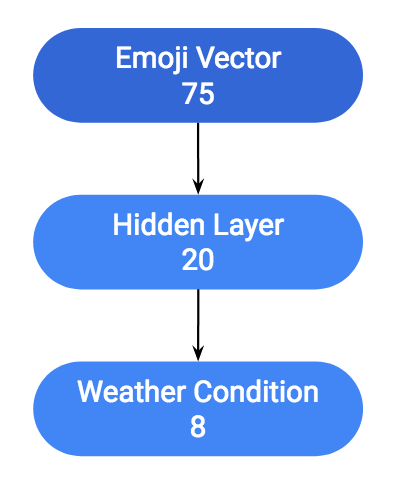
\includegraphics[scale=0.7]{neuralnet}
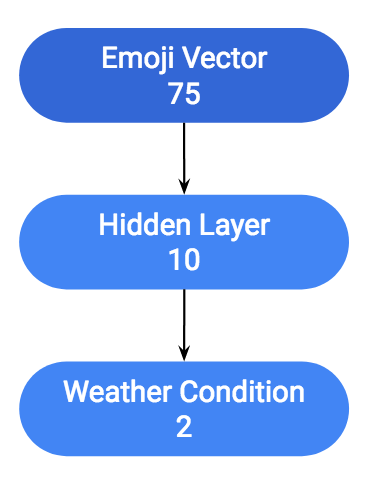
\includegraphics[scale=0.7]{neuralnetbinary}
\centering
\caption{Structure of our artificial neural networks. \textbf{Left:} ANN for standard classification. \textbf{Right:} ANN for binary classification. The numbers below the name of each layer represents the number of nodes in the layer.}
\label{fig:neuralnet}
\end{figure}

\section{Results}\label{results}

\subsection{Binary Classification}
We first frame our problem as binary classification. We thought that a simpler form of classification may yield better results. A description of the two classes can be seen in section \ref{preprocessing}. The Gaussian Mixture Model performs the worst, at 51\%, indicating that the data does not cluster well. On average, ZeroR outperforms all of our other models, at 59\%. This indicates that the models are unable to learn a relationship between the emoji vectors and our two classes. Most likely, the limited success is due to the nature of the classes. Some atmospheric conditions that we label as negative might not belong in that class. For instance, snow may actually be a positive condition for some people, leading them to use happier emojis in their tweets. See Figure \ref{fig:binary} for a detailed breakdown of the accuracies associated with each model.

\begin{figure}[H]
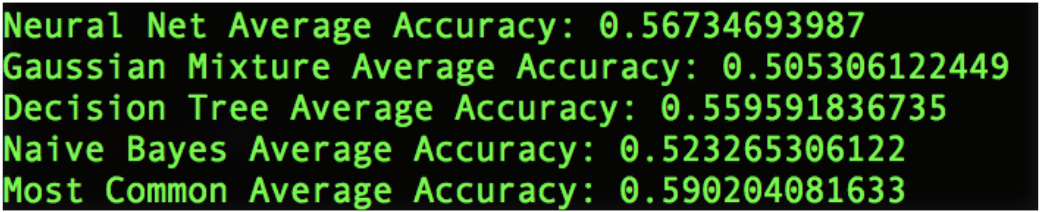
\includegraphics[scale=0.6]{binaryavg}
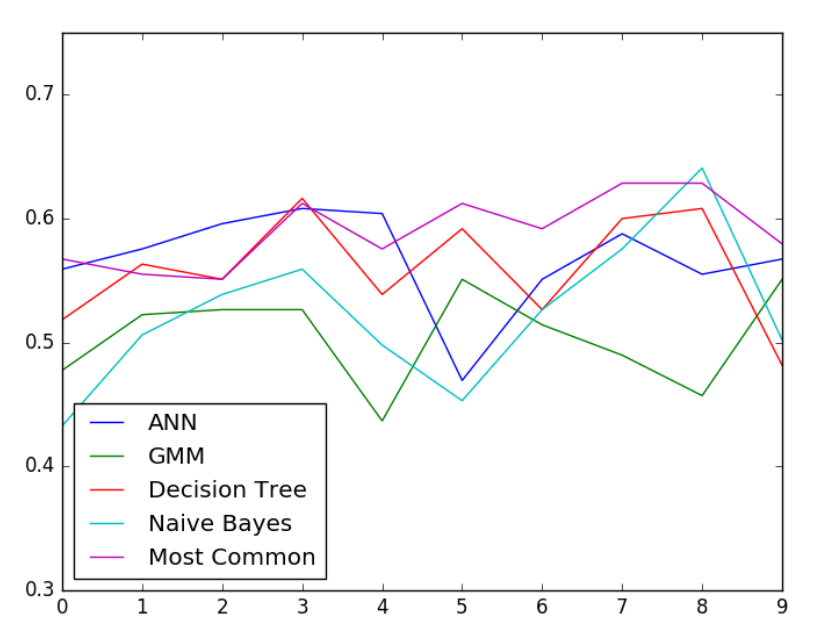
\includegraphics[scale=0.7]{binarygraph}
\centering
\caption{Binary classification results. \textbf{Top:} Average Accuracy for each model \textbf{Bottom:} Accuracy for each model over ten trials.}
\label{fig:binary}
\end{figure}

\subsection{Standard Classification}
We next framed our problem as a classification task with eight classes. A description of the classes can be seen in section \ref{preprocessing}. Here, Naive Bayes performs the worse, at 19\% accuracy. This is most likely due to the lack of statistical independence among emojis. Most notably, multiple emojis can come from the same tweet; such emojis are certainly not independent. The ANN significantly outperforms the other models, averaging 88\% accuracy. These results indicate that there does exist a relationship between emoji vectors and their atmospheric class. However, the relationship is too complex for models other than the ANN. Figure \ref{fig:standard} provides a detailed breakdown of the accuracy of each model. Figure \ref{fig:ann} provides the accuracy of the ANN on each of our 8 classes. The model does not just learn a few classes well, but achieves reasonable accuracy on all common classes.

\begin{figure}[H]
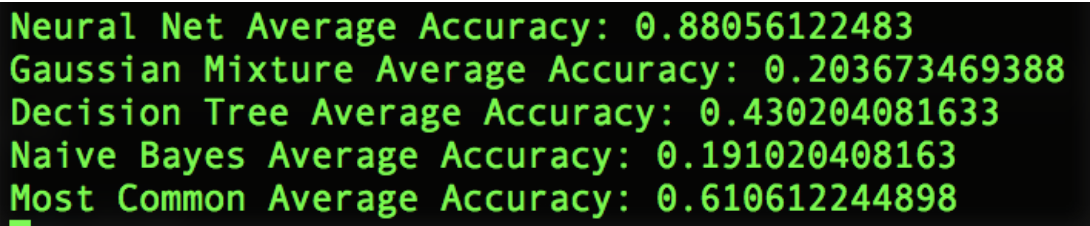
\includegraphics[scale=0.6]{standardavg}
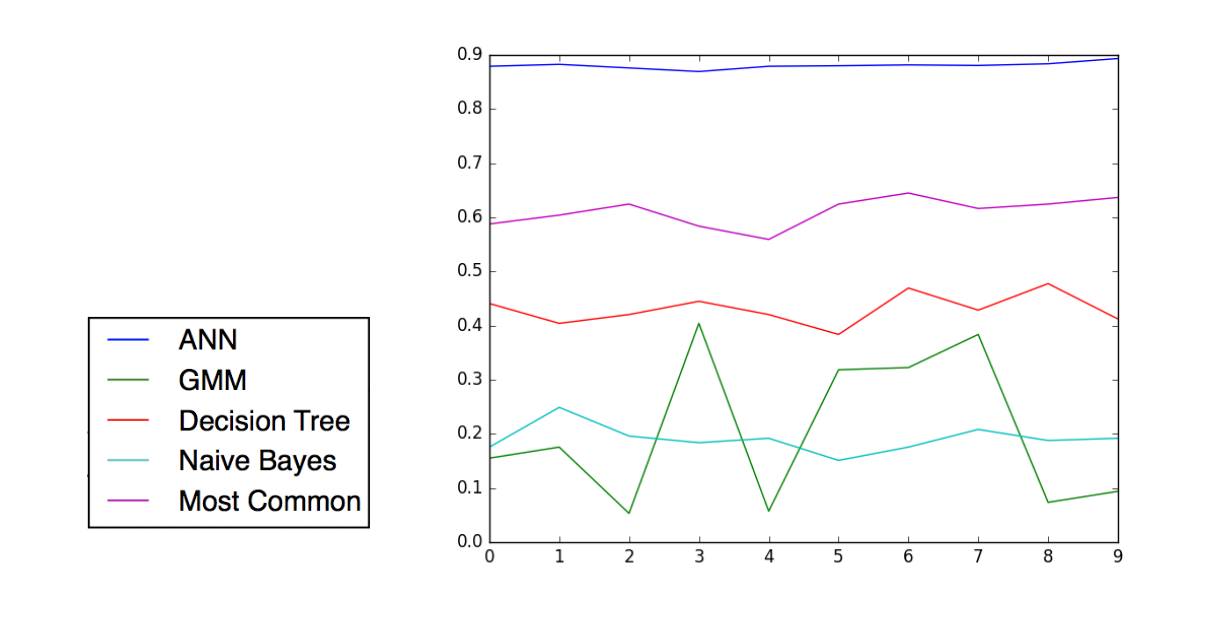
\includegraphics[scale=0.7]{standardgraph}
\centering
\caption{Standard classification results. \textbf{Top:} Average Accuracy for each model \textbf{Bottom:} Accuracy for each model over ten trials.}
\label{fig:standard}
\end{figure}

\begin{figure}[H]
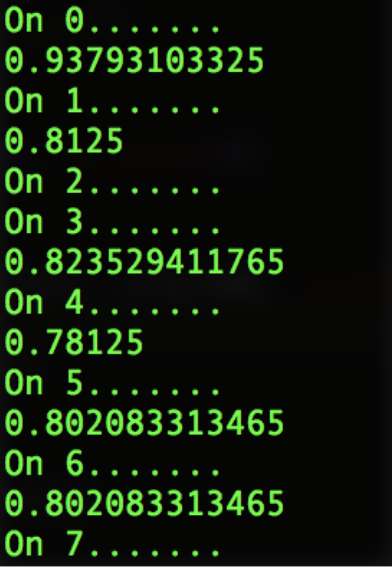
\includegraphics[scale=0.6]{ann}
\centering
\caption{Accuracy of the artificial neural network for each of our eight classes. Each classes integer value is printed, along with the percentage immediately below it.}
\label{fig:ann}
\end{figure}

\section{Conclusions}\label{conclusions}
Our results support the relationship between weather and emotion. Based upon the distribution of emojis used in a given city, our ANN was able to predict the atmospheric condition of that city with 88\% accuracy. Although our hypothesis was supported, we cannot draw specific conclusions regarding the relationship. To do this, further analysis is needed.

Most of the challenges that we encountered were related to the Twitter API. Initially, we believed that we could use prior tweets to generate our data. However, we learned that the Twitter API only allows you to collect tweets from the previous week. Furthermore, there is a cap on the number of tweets you can collect of 1500. We resolved this problem by collecting tweets in real time using the Twitter Streaming API. The consequences of collecting data this way was that we had to wait a couple weeks before we had any data to work with. Given the restricted time frame for the project, this limited the time that we could spend developing and evaluating our models.

Future work would involve determining which emojis have the strongest correlation with each weather condition. From this information, we could directly infer which emotions are elicited from each weather condition. We would also benefit from having a larger dataset. We could expand our scripts to gather tweets from all around the world with relative ease. This would also open up the possibility of analyzing the effect across cultures.

\bibliographystyle{plain}
\bibliography{emoji}

\end{document}
